%----------------------------------------------------------------------------------------
%	PACKAGES AND OTHER DOCUMENT CONFIGURATIONS
%----------------------------------------------------------------------------------------

\documentclass[12pt]{article}											% font size
\usepackage{subfig}
\usepackage{graphicx}													% to include images
\usepackage{float}														% to float figures
\usepackage{booktabs,makecell}											% for diagonal cells
\usepackage{hyperref}													% for hyperlinks
\usepackage{listings}													% for including files
\usepackage[top=1in, bottom=1in, left=1.25in, right=1.25in]{geometry}	% set margins
\usepackage[utf8]{inputenc}												% for unicode input characters
\usepackage{helvet}														% use helvetica per default
\usepackage{hyperref}													% for hyperlinks
\usepackage[T1]{fontenc}
\usepackage[english]{babel}
\usepackage{color}

\renewcommand{\familydefault}{\sfdefault}								% use sans serif per default

\definecolor{codegreen}{rgb}{0,0.6,0}									%New colors defined below
\definecolor{codegray}{rgb}{0.5,0.5,0.5}
\definecolor{codepurple}{rgb}{0.58,0,0.82}
\definecolor{backcolour}{rgb}{0.95,0.95,0.92}

\lstdefinestyle{mystyle}{												%Code listing style named "mystyle"
  backgroundcolor=\color{backcolour},   commentstyle=\color{codegreen},
  keywordstyle=\color{magenta},
  numberstyle=\tiny\color{codegray},
  stringstyle=\color{codepurple},
  basicstyle=\footnotesize,
  breakatwhitespace=false,         
  breaklines=true,                 
  captionpos=b,                    
  keepspaces=true,                 
  numbers=left,                    
  numbersep=5pt,                  
  showspaces=false,                
  showstringspaces=false,
  showtabs=false,                  
  tabsize=2
}

\lstset{style=mystyle}													%"mystyle" code listing set

% ----------------------------------------------------------------------------------------
%	TITLE SECTION 
% ----------------------------------------------------------------------------------------

\makeatletter
\makeatother
\renewcommand{\familydefault}{\sfdefault}								% use sans serif per default
\makeatother
\title{Usharesoft: Internship\\ PXE environment.   Designed architecture}
\author{Riyane SID-LAKHDAR}
\date{\today}


\begin{document}

\maketitle
\tableofcontents
\newpage




% ------------------------------------------------------------------------------
% No intermediate between client anf Uforge
% ------------------------------------------------------------------------------
\section{Software architecture 1: No intermediate between client anf Uforge}
\subsection{Client Grub interface:}
	\begin{enumerate}
		\item \textbf{"Secure Uforge choice":} Allows to access the PXE dedicated images on the client's Uforge account.   This item requires the user to enter his uforge credentials.   This option is automatically selected through a timeout system and requires no user action.
		\item \textbf{"Uforge default PXE os":} Allows to load the default os image set on Uforge (without any account needed).\\
		\item \textbf{"Local cache multi-choice":} Choosing this item allows to access a grub where to chose between different os images.   These images must be located on the "PXE server" cache.
	\end{enumerate}


% ------------------------------------------------------------------------------
\subsection{Global architecture}

	\begin{figure*}[t]
	\begin{center}
		\subfloat[Architecture]
		{
			\includegraphics[width=0.5\hsize]{chart/architecture_noIntermediary.png}
		}
		\subfloat[Network flow diagram]
		{
			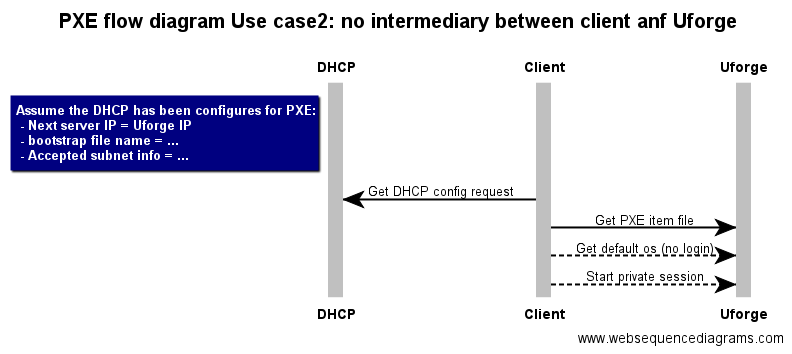
\includegraphics[width=0.5\hsize]{chart/flowDiagram_noIntermediary.png}
		}
		\caption{Representation of the solution 2: no intermediary between uforge and client hosts.}
	\end{center}
	\end{figure*}


% ------------------------------------------------------------------------------
\subsection{Advantages}
	\begin{itemize}
		\item No need for the client to install or download any new tool (on his network or central server).
		\item All the improvement and the upgrades may be proposed without any intervention of the user: all the binaries and scripts that uses the user are provided at boot time.
	\end{itemize}
   


% ------------------------------------------------------------------------------
\subsection{Drawbacks}
	\begin{enumerate}
		\item Very few features may be added for the client network side.
		\item A same file may be sent several times by uforge to the same network hence contention on uforge server.  It also downgrades the performances for the client.
	\end{enumerate}








% ------------------------------------------------------------------------------
% Proxy/Cache between Uforge and client host
% ------------------------------------------------------------------------------
\section{Software architecture 2: Proxy/Cache between Uforge and client host}
\subsection{Client Grub interface:}
	\begin{enumerate}
		\item \textbf{"Private session":} Allows to access the PXE dedicated images on the client's Uforge account.   This item requires the user to enter his uforge credentials.   This option is automatically selected through a timeout system and requires no user action.
		\item \textbf{"Uforge default PXE os":} Allows to load the default os image set on the central proxy server.\\
		\item \textbf{"Cached multi-choice":} Choosing this item allows to access a grub where to chose between different os images.   These images must be located on the "PXE server" cache.   They must have been declared by the central proxy as accessible for your IP (or sub network).
	\end{enumerate}


% ------------------------------------------------------------------------------
\subsection{Global architecture}

	\begin{figure*}[t]
	\begin{center}
		\subfloat[Architecture]
		{
			\includegraphics[width=0.5\hsize]{chart/architecture_proxy.png}
		}
		\subfloat[Network flow diagram]
		{
			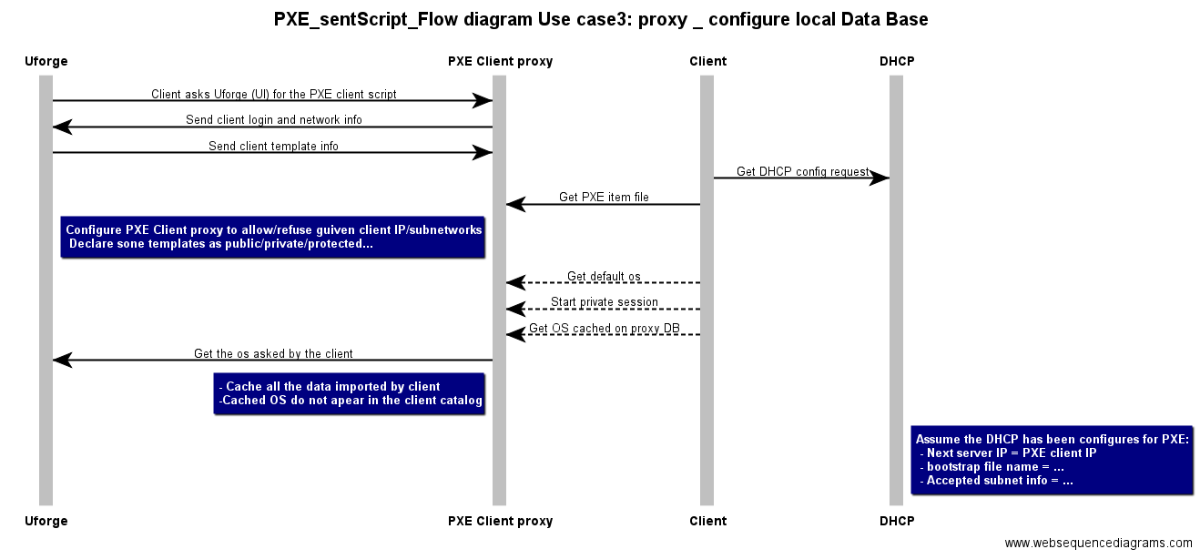
\includegraphics[width=0.5\hsize]{chart/flowDiagram_proxy.png}
		}
		\caption{Representation of the solution 3: proxy between Uforge and client hosts.}
	\end{center}
	\end{figure*}


% ------------------------------------------------------------------------------
\subsection{Advantages}
	First, this architecture reduces the contention on the uforge server: the the same template may be sent only once for different users (cache on the client Cache).   Thus, the client has also a better time performance as most exchanges are done within his local network.\\

	Second, we may allow the user to automatize some installation tasks on his network:  he may define the templates that he wants to open.  He may also define the groups or sub groups that access to each template.


% ------------------------------------------------------------------------------
\subsection{Drawbacks}
	\begin{enumerate}
		\item Very few features may be added for the client network side.
		\item A same file may be sent several times by uforge to the same network hence contention on uforge server.  It also downgrades the performances for the client.
	\end{enumerate}


% ------------------------------------------------------------------------------
% Implementations
% ------------------------------------------------------------------------------
\section{Implementations}
\subsection{iPXE web-resources (integrated to UForge)}
	In order to answer to the pxe request, we have implemented three web-resources integrated within the UForge environment:
    \begin{itemize}
		\item The class "NonAuthentifiedResource.java" allows to get all the PXE binaries and the PXE script that a light user may need before it is able to log to UForge.   This web-resource does not requires any authentication.   2 rest URI are linked to this web-resource (see section \ref{resource_noAuthentication_script}, and \ref{resource_noAuthentication_defaultImage}).
		\item The class "UserImagesResource.java" allows to get the PXE script that prints the prints the interface during a private session (see section \ref{privateSessionScript}).   This script is built dynamically using the dynamic code generation tools ().
        \item The class "ApplianceDownloadResource.java" has been modified to allow to download independent files of an ISO which may have a path of depth higher than 1.
	\end{itemize}


% ------------------------------------------------------------------------------
\subsection{Dynamic code generation tool (used by the web-resources)} \label{codeGenerationTool}
	In order to dynamically build the PXE scripts that are sent to the user, we have implemented the tool "ScriptCreator" within the UForge environment (uForgeRest.com.usharesoft.rest.utils).\\
	This use an initial code template that is parsed using a state automaton looking for some key words.   Each key word is mapped to one of the actions: write string, loop on an other template, call a function. 


% ------------------------------------------------------------------------------
\subsection{Scripts to set an iPXE environment on an independent server}
	In order to set an iPXE environment, we have implemented the script "setPxeEnvironment/setPxeServer.sh".   The options of this tool may be discovered thanks to the option "-help".   This script allows to configure and run different services needed by the PXE specification:
	\begin{itemize}
		\item Configure and launch the DHCP and DNS servers (see section \ref{dhcp_dns_configFile}).
		\item Configure and launch a tftp server (in order to send the initial iPXE binary).
		\item Configure and launch an HTTP server (to execute all the other file exchanges).
		\item Populate the http server (or TFTP in case of exclusive PXE) with the sysloader binaries (required by the installer).
		\item Populate the http server (or TFTP in case of exclusive PXE) with the os files (iso that has been mounted).
	\end{itemize}
	Different scripts have been implemented to automatize all this processes.   They may all be found in "setPxeEnvironment/util".


% ------------------------------------------------------------------------------
\subsection{Example of outputs}
	\subsubsection{iPXE scripts}
	An example of each script has been put in the directory "examples/pxeScript".   This files may be sent as is to the light user in order to print a specific interface.   Each one of this script has been dynamically generated by a UForge web-resources as an answer to a specific PXE request.   The name of the web-resource java class and the context of the generations are indicated on the head of each file. 

	\subsubsection{DHCP/DNS configuration file} \label{dhcp_dns_configFile}
	An example of DHCP and DNS configuration files has been put in the directories "examples/dhcpConfig" and "examples/dnsConfig".   This configuration files has been respectively used with "dhcpd" and "dnsmasq".


% ------------------------------------------------------------------------------
% GENERAL NOTES IPXE
% ------------------------------------------------------------------------------
\section{General notes}
\subsection{Issues to boot on a UForge-generated centos7 ISO with a PXE environment}
	The iso generated on UForge did not boot till the end using the PXE environment.   It stopped during the installation (done by the "anaconda" boot loader after the kernel and file system have been downloaded).\\
	Two issues have been noticed during the installation:
	\begin{itemize}
		\item A warning has been shown by the installer indicating the the package \textit{\textbf{"kexec-tools"}} has been specified in the profile but does not exist in the iso (see figure \ref{installer_warning_kexec-tools}).  This warning is probably due to a bug during the iso generation (on Uforge) as this package doesn't appear in the required package list (seen on the UForge UI).   This warning may be ignored.
		\item A fatal error has been shown by the installer indicating the the package \textit{\textbf{"xfsprogs"}} is mandatory for the installer to succeed but does not exist in the iso (see figure \ref{installer_error_xfsprogs}).
	\end{itemize}
	This issues have been fixed by simply adding the previous two packages to the used iso (within the install profile on the Uforge user-interface).

	\begin{figure*}[t]
	\begin{center}
		\subfloat[Installer warning]
		{
			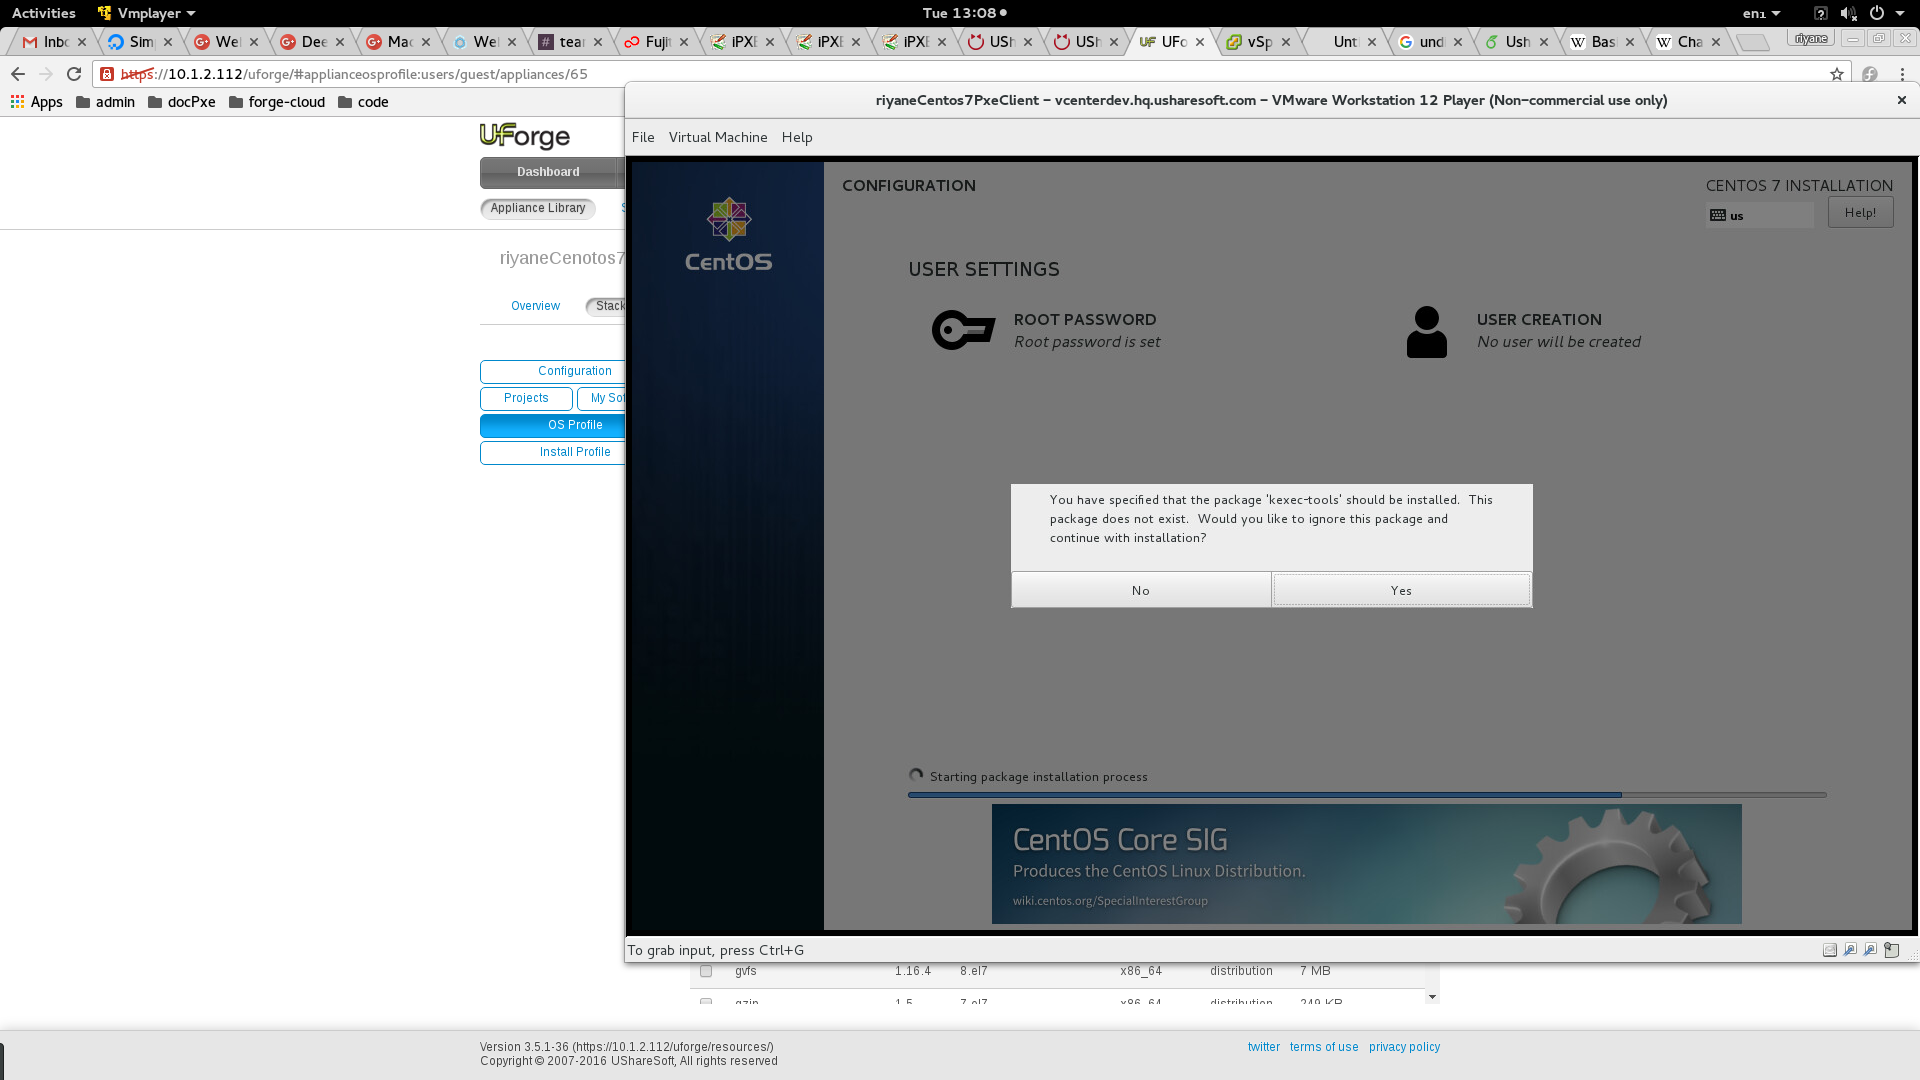
\includegraphics[width=0.5\hsize]{chart/uforgeIso_missingLibrary_kexec-tools_warning.png}
        	\label{installer_warning_kexec-tools}
		}
		\subfloat[Installer fatal error]
		{
			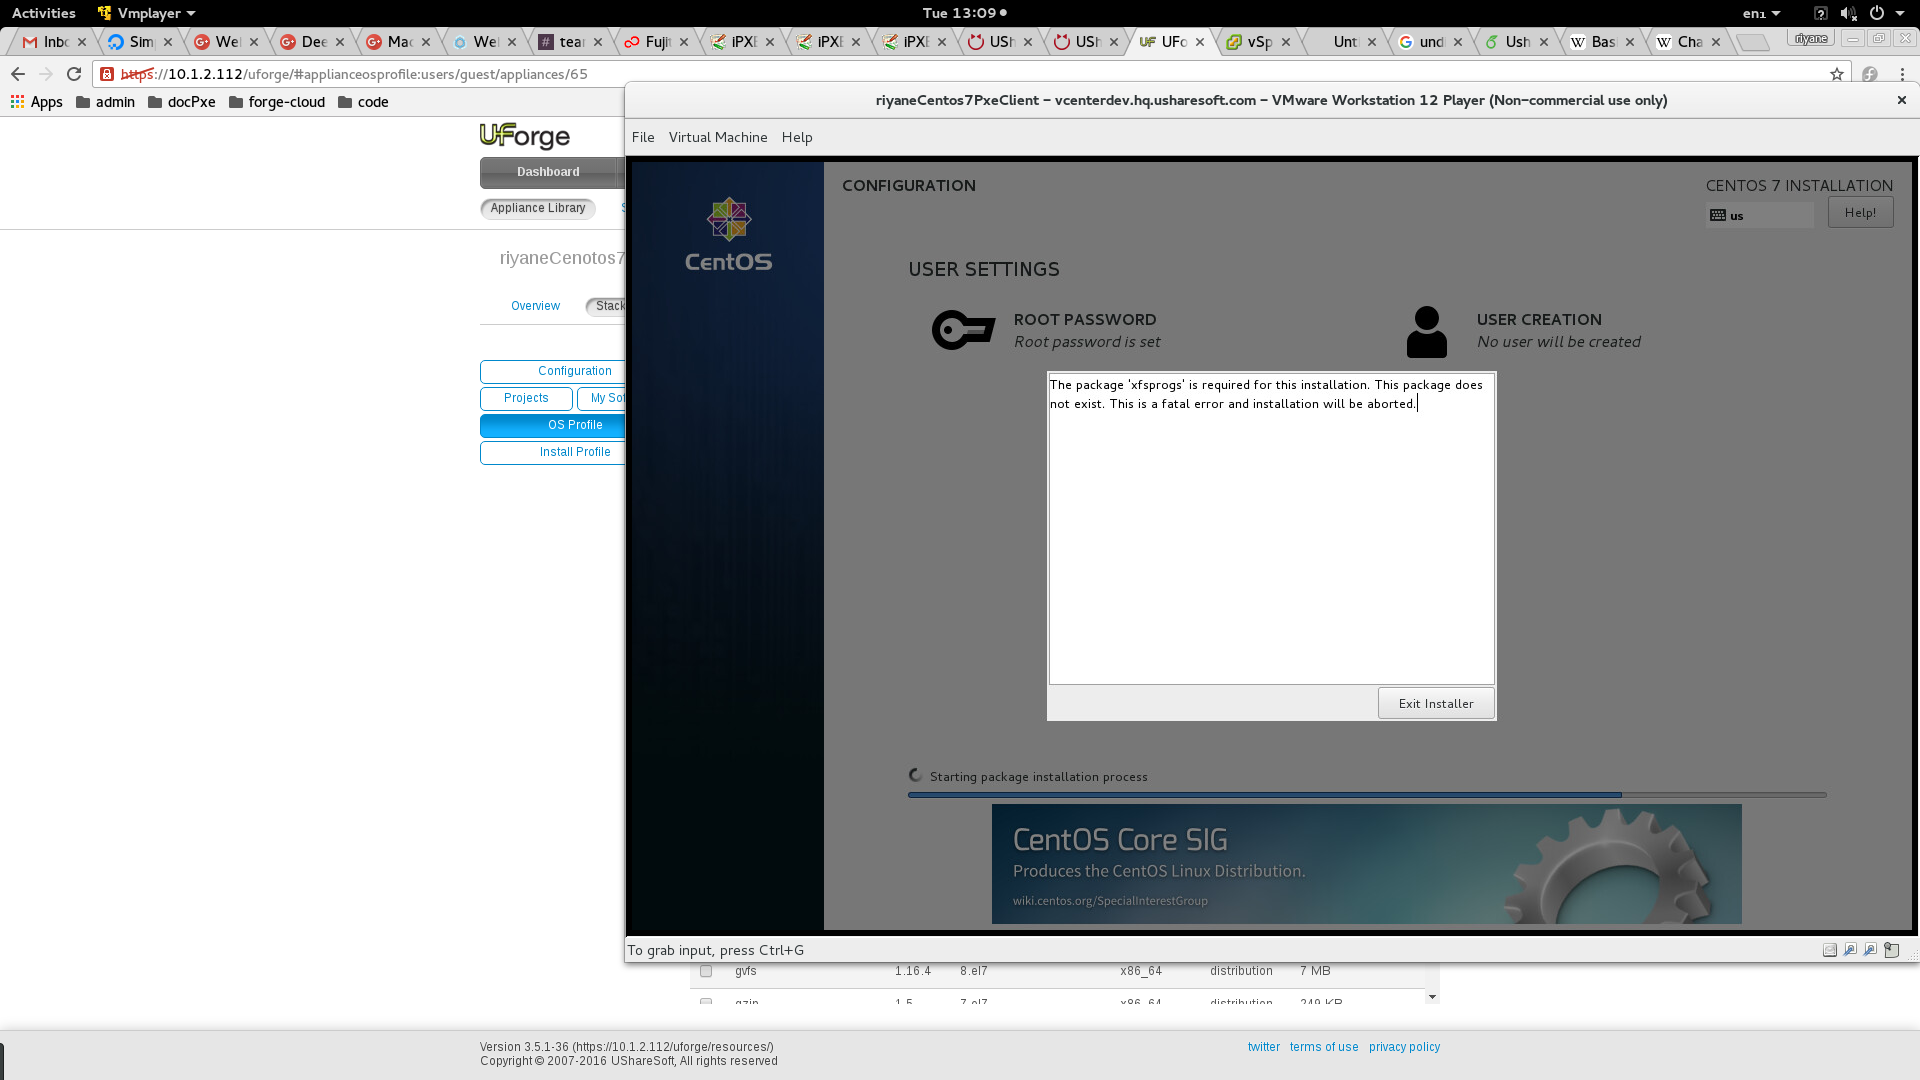
\includegraphics[width=0.5\hsize]{chart/uforgeIso_missingLibrary_xfsprogs_error.png}
            \label{installer_error_xfsprogs}
		}
		\caption{Missing packages in the Uforge generated iso}
	\end{center}
	\end{figure*}


% ------------------------------------------------------------------------------
\subsection{Issues to boot on a UForge-generated Ubuntu-14.04 ISO with a PXE environment}
The problem with this iso is that the path to the kernel (vmlinuz) and the file system (initrd.img) are not the one expected by the boot loader.   This issue has been corrected by simply replace them ones the ISO has been mounted at "images/pxeboot/"


% ------------------------------------------------------------------------------
\subsection{Build the iPXE binary}\label{buildIpxeBinary}
	The ipxe binary that is initially sent to the user has been build based on the open source firmware iPxe (see http://ipxe.org/).\\
	In order to download this firmware, we have implemented the script ipxeFirmware/setIpxeFirmware.sh.\\
    Then, to build the final iPxe binary, we need to into the generated directory "ipxe/ipxe-bios/src" and run the command\\ \textbf{" make bin/undionly.kpxe HTTP\_AUTH\_BASIC=enable DOWNLOAD\_PROTO\_HTTPS=enable EMBED=<pxeInitialScript> "}\\
    where "pxeInitialScript" is the script that you can find at "setpxeEnvironment/config/pxeConf.d/bootstrapScript.ipxe.initial".\\
	Note that a requirement to this build process is to have the packages "zlib-devel" and "binutils-devel".


% ------------------------------------------------------------------------------
\subsection{General resource (not managed by the web-resource)}
	\subsubsection{Resource iPXE binary}
		\begin{itemize}
			\item \textbf{\textit{Type:}} TFTP
			\item \textbf{\textit{URL:}} undionly.kpxe
			\item \textbf{\textit{Return:}} The initial iPXE binary.
			\item \textbf{\textit{Details:}} This initial binary (iPXE binary) is supposed to replace the initial PXE binary which was by default burned on the light client network card ROM.  It needs to be build according to the process described section \ref{buildIpxeBinary}.\\
            This binary needs to be accessed by all the clients without any authentication.   It also needs to be build and configured for the destination client processor architecture.
		\end{itemize}


% ------------------------------------------------------------------------------
	\subsection{REST resource with no authentication (managed by the web-resource)}
		\subsubsection{iPXE script (main menu / private session specific to image)} \label{resource_noAuthentication_script}
			\begin{itemize}
				\item \textbf{\textit{Type:}} HTTP GET
				\item \textbf{\textit{URL:}} noAuthentication/pxeScriptResource/\{sn\}
				\item \textbf{\textit{Parameter:}}
					\begin{itemize}
						\item sn: Name of the script to download (may be a path with sevral sub directories)
					\end{itemize}
				\item \textbf{\textit{Return:}} The iPXE script that prints the main menu or the menu for a private session (specific to an image)
				\item \textbf{\textit{Details:}} This script must allow to print the main menu of the iPXE interface.   For each item of the menu, it must indicate the correct resource.   No authentication is required to access this resource.
			\end{itemize}

		\subsubsection{Default PXE OS (get independent files of the OS)} \label{resource_noAuthentication_defaultImage}
			\begin{itemize}
				\item \textbf{\textit{Type:}} HTTP GET
				\item \textbf{\textit{URL:}} noAuthentication/pxeDefaultImage/\{os-fileName++\}
				\item \textbf{\textit{Parameter:}}
					\begin{itemize}
						\item os-fileName: Path to a file of the default os.  May be a path with several sub-directories
					\end{itemize}
				\item \textbf{\textit{Return:}} A file belonging to the default os.
				\item \textbf{\textit{Details:}} No authentication is required.
			\end{itemize}


% ------------------------------------------------------------------------------

	\subsection{REST resource with authentication (managed by the web-resource)}
		\subsubsection{User-specific PXE OS (independent files of the OS)} \label{userSpecificImagePxeScript}
			\begin{itemize}
				\item \textbf{\textit{Type:}} HTTP GET
				\item \textbf{\textit{URL:}} /users/\{uid\}/appliances/\{aid\}/images/\{itid\}/downloads/\{os-fileName++\}
				\item \textbf{\textit{Parameter:}}
					\begin{itemize}
						\item uid: user id (UForge login)
						\item aid: Appliance id
                        \item itid: image id
                        \item os-fileName: OS file name.   May be a path with several sub-directories.
					\end{itemize}
				\item \textbf{\textit{Return:}} The iPXE script that prints the list of os accessible by the user after he is logged.
				\item \textbf{\textit{Details:}} This request is sent after the user has logged him self.   
			\end{itemize}


% ------------------------------------------------------------------------------

	\subsubsection{iPXE script for a private session} \label{privateSessionScript}
		\begin{itemize}
			\item \textbf{\textit{Type:}} HTTP GET
			\item \textbf{\textit{URL:}} /users/{uid}/images/scriptPxePrivateSession
			\item \textbf{\textit{Parameter:}}
				\begin{itemize}
					\item Uid: UForge login of the user
				\end{itemize}
			\item \textbf{\textit{Return:}} The iPXE script that prints all the accessible PXE images for the given user.
			\item \textbf{\textit{Details:}} This script must allow to print all the accessible images for the current user.   For each item of the menu, it must indicate the correct resource \ref{userSpecificImagePxeScript}.   An authentication is required.
		\end{itemize}


\end{document}